\documentclass{if-beamer}

% --------------------------------------------------- %
%                  Presentation info	              %
% --------------------------------------------------- %
\title[Lecture 23]{Integration}
\subtitle{Adaptive Quadrature}
\author{Ashley Gannon}
\date{Fall 2020}
\logo{

\includegraphics[scale=0.08]{figures/FSULogo.png}
}
\subject{Presentation subject}

% --------------------------------------------------- %
%                    Title + Schedule                 %
% --------------------------------------------------- %
\begin{document}

\begin{frame}
  \titlepage
\end{frame}
% --------------------------------------------------- %
%                      Presentation                   %
% --------------------------------------------------- %
\section{Adaptive Quadrature}

\begin{frame}[t]
	\frametitle{Adaptive Quadrature}
	While Romberg integration is more efficient than the composite Simpson's 1/3 rule, both methods use equispaced points.  \\\vspace{7pt}
	
\end{frame}


\begin{frame}[t]
\frametitle{Adaptive Quadrature}
While Romberg integration is more efficient than the composite Simpson's 1/3 rule, both methods use equispaced points.  \\\vspace{7pt}

This constraint does not take into account that some functions have regions of relatively abrupt changes where more refined spacing might be
required.
\end{frame}

\begin{frame}[t]
	\frametitle{Adaptive Quadrature}
	While Romberg integration is more efficient than the composite Simpson's 1/3 rule, both methods use equispaced points.  \\\vspace{7pt}
	
	This constraint does not take into account that some functions have regions of relatively abrupt changes where more refined spacing might be
	required.
	\begin{itemize}
		\item These methods require that fine spacing be applied everywhere on the domain even though it is only needed for the regions of sharp change
	\end{itemize}
	
	\begin{figure}
		\centering
		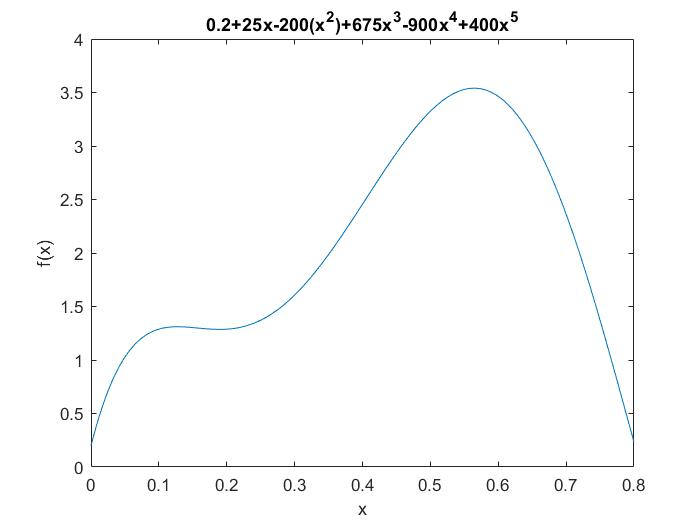
\includegraphics[width = 0.4\textwidth]{figures/example}
	\end{figure}
\end{frame}

\begin{frame}[t]
	\frametitle{Adaptive Quadrature}
	While Romberg integration is more efficient than the composite Simpson's 1/3 rule, both methods use equispaced points.  \\\vspace{7pt}
	
	This constraint does not take into account that some functions have regions of relatively abrupt changes where more refined spacing might be
	required.
	\begin{itemize}
		\item These methods require that fine spacing be applied everywhere on the domain even though it is only needed for the regions of sharp change
	\end{itemize}
	
	\begin{figure}
		\centering
		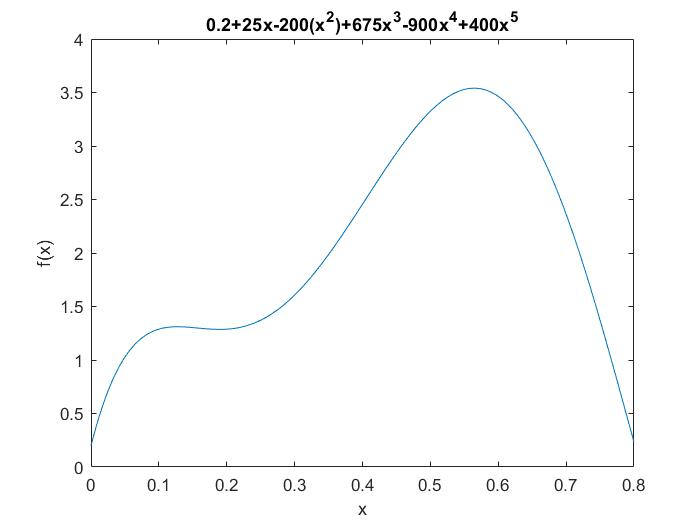
\includegraphics[width = 0.4\textwidth]{figures/example}
	\end{figure}
	Adaptive quadrature methods remedy this situation by automatically adjusting the step size so that small steps are taken in regions of sharp variations and larger steps are taken where the function changes gradually.
\end{frame}

\begin{frame}[t]
	\frametitle{Adaptive Quadrature}
	Adaptive quadrature methods accommodate the fact that many functions have regions of
	high variability along with other sections where change is gradual.
\end{frame}

\begin{frame}[t]
	\frametitle{Adaptive Quadrature}
	Adaptive quadrature methods accommodate the fact that many functions have regions of
	high variability along with other sections where change is gradual.
	\begin{itemize}
		\item They accomplish this
		by adjusting the step size so that small intervals are used in regions of rapid variations and
		larger intervals are used where the function changes gradually. \vspace{5pt}
	\end{itemize}
\end{frame}

\begin{frame}[t]
	\frametitle{Adaptive Quadrature}
	Adaptive quadrature methods accommodate the fact that many functions have regions of
	high variability along with other sections where change is gradual.
	\begin{itemize}
		\item They accomplish this
		by adjusting the step size so that small intervals are used in regions of rapid variations and
		larger intervals are used where the function changes gradually. \vspace{5pt}
		\item Many of these techniques
		are based on applying the composite Simpson’s 1/3 rule to subintervals in a fashion that
		is very similar to the way in which the composite trapezoidal rule was used in Richardson
		extrapolation. \vspace{5pt}
	\end{itemize}
\end{frame}

\begin{frame}[t]
	\frametitle{Adaptive Quadrature}
	Adaptive quadrature methods accommodate the fact that many functions have regions of
	high variability along with other sections where change is gradual.
	\begin{itemize}
		\item They accomplish this
		by adjusting the step size so that small intervals are used in regions of rapid variations and
		larger intervals are used where the function changes gradually. \vspace{5pt}
		\item Many of these techniques
		are based on applying the composite Simpson’s 1/3 rule to subintervals in a fashion that
		is very similar to the way in which the composite trapezoidal rule was used in Richardson
		extrapolation. \vspace{5pt}
		\begin{itemize}
			\item The 1/3 rule is applied at two levels of refinement, and the difference
			between these two levels is used to estimate the truncation error. \vspace{3pt}
		\end{itemize}
	\end{itemize}
\end{frame}


\begin{frame}[t]
	\frametitle{Adaptive Quadrature}
	Adaptive quadrature methods accommodate the fact that many functions have regions of
	high variability along with other sections where change is gradual.
	\begin{itemize}
		\item They accomplish this
		by adjusting the step size so that small intervals are used in regions of rapid variations and
		larger intervals are used where the function changes gradually. \vspace{5pt}
		\item Many of these techniques
		are based on applying the composite Simpson’s 1/3 rule to subintervals in a fashion that
		is very similar to the way in which the composite trapezoidal rule was used in Richardson
		extrapolation. \vspace{5pt}
		\begin{itemize}
			\item The 1/3 rule is applied at two levels of refinement, and the difference
			between these two levels is used to estimate the truncation error. \vspace{3pt}
			\item If the truncation error is
			acceptable, no further refinement is required, and the integral estimate for the subinterval is
			deemed acceptable. \vspace{3pt}
		\end{itemize}
	\end{itemize}
\end{frame}

\begin{frame}[t]
	\frametitle{Adaptive Quadrature}
	Adaptive quadrature methods accommodate the fact that many functions have regions of
	high variability along with other sections where change is gradual.
	\begin{itemize}
		\item They accomplish this
		by adjusting the step size so that small intervals are used in regions of rapid variations and
		larger intervals are used where the function changes gradually. \vspace{5pt}
		\item Many of these techniques
		are based on applying the composite Simpson’s 1/3 rule to subintervals in a fashion that
		is very similar to the way in which the composite trapezoidal rule was used in Richardson
		extrapolation. \vspace{5pt}
		\begin{itemize}
			\item The 1/3 rule is applied at two levels of refinement, and the difference
			between these two levels is used to estimate the truncation error. \vspace{3pt}
			\item If the truncation error is
			acceptable, no further refinement is required, and the integral estimate for the subinterval is
			deemed acceptable. \vspace{3pt}
			\item  If the error estimate is too large, the step size is refined and the process
			repeated until the error falls to acceptable levels \vspace{3pt}
		\end{itemize}
	\end{itemize}
\end{frame}

\begin{frame}[t]
	\frametitle{Adaptive Quadrature}
	Adaptive quadrature methods accommodate the fact that many functions have regions of
	high variability along with other sections where change is gradual.
	\begin{itemize}
		\item They accomplish this
		by adjusting the step size so that small intervals are used in regions of rapid variations and
		larger intervals are used where the function changes gradually. \vspace{5pt}
		\item Many of these techniques
		are based on applying the composite Simpson’s 1/3 rule to subintervals in a fashion that
		is very similar to the way in which the composite trapezoidal rule was used in Richardson
		extrapolation. \vspace{5pt}
		\begin{itemize}
			\item The 1/3 rule is applied at two levels of refinement, and the difference
			between these two levels is used to estimate the truncation error. \vspace{3pt}
			\item If the truncation error is
			acceptable, no further refinement is required, and the integral estimate for the subinterval is
			deemed acceptable. \vspace{3pt}
			\item  If the error estimate is too large, the step size is refined and the process
			repeated until the error falls to acceptable levels \vspace{3pt}
			\item The total integral is then computed as the
			summation of the integral estimates for the subintervals.
		\end{itemize}
	\end{itemize}
\end{frame}

\begin{frame}[t]
	\frametitle{Adaptive Quadrature}
	In theory, if we have the interval $x \in [a,b]$ with a width of $h_1 = b-a$, a first estimate with Simpson's 1/3 rule can be computed using
	$$ I(h_1) = \frac{h_1}{6}(f(a) + 4f(c) + f(b))$$ 
	where $c = (a+b)/2$. \\\vspace{5pt}
\end{frame}

\begin{frame}[t]
	\frametitle{Adaptive Quadrature}
	In theory, if we have the interval $x \in [a,b]$ with a width of $h_1 = b-a$, a first estimate with Simpson's 1/3 rule can be computed using
	$$ I(h_1) = \frac{h_1}{6}(f(a) + 4f(c) + f(b))$$ 
	where $c = (a+b)/2$. \\\vspace{5pt}
	As we did with Richardson Extrapolation, a more refined estimate can be computed by halving the interval, $h_2 = h_1/2 = (b-a)/2$
	$$I(h_2) =\frac{h_2}{6}(f(a) +4f(d) +2f(c) +4f(e) +f(b))$$
	where $d = (a+c)/2$ and $e = (c+b)/2$. 
\end{frame}

\begin{frame}[t]
	\frametitle{Adaptive Quadrature}
	In theory, if we have the interval $x \in [a,b]$ with a width of $h_1 = b-a$, a first estimate with Simpson's 1/3 rule can be computed using
	$$ I(h_1) = \frac{h_1}{6}(f(a) + 4f(c) + f(b))$$ 
	where $c = (a+b)/2$. \\\vspace{5pt}
	As we did with Richardson Extrapolation, a more refined estimate can be computed by halving the interval, $h_2 = h_1/2 = (b-a)/2$
	$$I(h_2) =\frac{h_2}{6}(f(a) +4f(d) +2f(c) +4f(e) +f(b))$$
	where $d = (a+c)/2$ and $e = (c+b)/2$. 
	Because both $I(h_1)$ and $I(h_2)$ are both estimates of the same integral, their difference can be used to measure the error of approximation
	$$ E \cong |I(h_2) -I(h_1)|$$ 
\end{frame}


\begin{frame}[t]
	\frametitle{Adaptive Quadrature}
	In addition, the estimate and error associated with either application can be represented generally as 
	$$I = I(h_n) +E(h_n)$$
	where $I$ is the exact integral, $I(h_n)$ is the approximate integral, $E(h_n)$ is the truncation error. \\\vspace{5pt}

\end{frame}

\begin{frame}[t]
	\frametitle{Adaptive Quadrature}
	In addition, the estimate and error associated with either application can be represented generally as 
	$$I = I(h_n) +E(h_n)$$
	where $I$ is the exact integral, $I(h_n)$ is the approximate integral, $E(h_n)$ is the truncation error. \\\vspace{5pt}
	Using a similar approach to what we did for Richardson extrapolation, we can derive an estimate in the error of the more refined estimate $I(h_2)$ as a function of the difference between the two integral estimates so that 
	$$E(h_2)= \frac{1}{15}\left(I(h_2)-I(h_1)\right)$$
\end{frame}

\begin{frame}[t]
	\frametitle{Adaptive Quadrature}
	In addition, the estimate and error associated with either application can be represented generally as 
	$$I = I(h_n) +E(h_n)$$
	where $I$ is the exact integral, $I(h_n)$ is the approximate integral, $E(h_n)$ is the truncation error. \\\vspace{5pt}
	Using a similar approach to what we did for Richardson extrapolation, we can derive an estimate in the error of the more refined estimate $I(h_2)$ as a function of the difference between the two integral estimates so that 
	$$E(h_2)= \frac{1}{15}\left(I(h_2)-I(h_1)\right)$$
	Which can be substituted into the general formula above, 
	$$I = I(h_2) +  \frac{1}{15}\left(I(h_2)-I(h_1)\right)$$
	This formula is known as \textit{Boole's rule}.
\end{frame}

\begin{frame}[t]
	\frametitle{Adaptive Quadrature}
	These equations can be combined into an efficient algorithm.

\end{frame}

\begin{frame}[t]
	\frametitle{Adaptive Quadrature}
	These equations can be combined into an efficient algorithm.
	\begin{itemize}
		\item Evaluate the initial application of Simpson's 1/3 rule by computing the two integral estimates
		\begin{align*}
		I(h_1) &= \frac{h_1}{6}(f(a) + 4f(c) + f(b))\\
		I(h_2) &=\frac{h_2}{6}(f(a) +4f(d) +2f(c) +4f(e) +f(b))\\
		\end{align*}
	\end{itemize}
\end{frame}

\begin{frame}[t]
	\frametitle{Adaptive Quadrature}
	These equations can be combined into an efficient algorithm.
	\begin{itemize}
		\item Evaluate the initial application of Simpson's 1/3 rule by computing the two integral estimates
		\begin{align*}
			I(h_1) &= \frac{h_1}{6}(f(a) + 4f(c) + f(b))\\
			I(h_2) &=\frac{h_2}{6}(f(a) +4f(d) +2f(c) +4f(e) +f(b))\\
		\end{align*}
		\item Estimate the error using the absolute difference between the two integral estimates, $|f(h_2)-f(h_1)|$. 
	\end{itemize}
\end{frame}

\begin{frame}[t]
	\frametitle{Adaptive Quadrature}
	These equations can be combined into an efficient algorithm.
	\begin{itemize}
		\item Evaluate the initial application of Simpson's 1/3 rule by computing the two integral estimates
		\begin{align*}
			I(h_1) &= \frac{h_1}{6}(f(a) + 4f(c) + f(b))\\
			I(h_2) &=\frac{h_2}{6}(f(a) +4f(d) +2f(c) +4f(e) +f(b))\\
		\end{align*}
		\item Estimate the error using the absolute difference between the two integral estimates, $|f(h_2)-f(h_1)|$.
		\item Depending on the error, one of two things will happen
		\begin{enumerate}
			\item If the error is less than or equal to the tolerance, we estimate the integral using Boole's rule:
			$$I = I(h_2) +\frac{1}{15}\left(I(h_2) -I(h_1)\right)$$
			\item If the error is larger than the tolerance, \texttt{AdaptiveQuadrature} is recursively called for each subinterval, $[a,c]$ and $[c,b]$. 
		\end{enumerate} 
	\end{itemize}
\end{frame}

\begin{frame}[t]
	\frametitle{Adaptive Quadrature}
	These equations can be combined into an efficient algorithm.
	\begin{itemize}
		\item Evaluate the initial application of Simpson's 1/3 rule by computing the two integral estimates
		\begin{align*}
			I(h_1) &= \frac{h_1}{6}(f(a) + 4f(c) + f(b))\\
			I(h_2) &=\frac{h_2}{6}(f(a) +4f(d) +2f(c) +4f(e) +f(b))\\
		\end{align*}
		\item Estimate the error using the absolute difference between the two integral estimates, $|f(h_2)-f(h_1)|$.
		\item Depending on the error, one of two things will happen
		\begin{enumerate}
			\item If the error is less than or equal to the tolerance, we estimate the integral using Boole's rule:
			$$I = I(h_2) +\frac{1}{15}\left(I(h_2) -I(h_1)\right)$$
			\item If the error is larger than the tolerance, \texttt{AdaptiveQuadrature} is recursively called for each subinterval, $[a,c]$ and $[c,b]$. 
		\end{enumerate} 
	\end{itemize}
	The beauty of this algorithm is in the two recursive calls. This recursion allows us to keep subdividing the intervals until our tolerance is met.
\end{frame}

\begin{frame}
	\frametitle{Adaptive Quadrature Pseudocode}
	\texttt{Define function that takes in a, b, and tol}\\
	\texttt{Declare/define h1 = b-a}\\
	\texttt{Declare/define h2 = h1/2}\\
	\texttt{Declare/define midpoints: }\\
	\texttt{\quad c = (a+b)/2}\\
	\texttt{\quad d = (a+c)/2}\\
	\texttt{\quad e = (c+b)/2} \\
	\texttt{Declare/define I}\\
	\texttt{ }\\
	\texttt{Declare/define Ih1 and Ih2}\\
	\texttt{\quad Ih1 = (h1/6)*(f(a)+4*f(c)+f(b))}\\
	\texttt{\quad Ih2 = (h2/6)*(f(a)+4*f(d) +2*f(c)+ 4*f(e) +f(b))}\\
	\texttt{ }\\ 
	\texttt{Declare/define the error}\\
	\texttt{error = abs(Ih2-Ih1)}\\
	\texttt{if error > tol}\\
	\texttt{\qquad Boole's Rule:}\\
	\texttt{\qquad I = Ih2 + (1/15)*(Ih2-Ih1)}\\
	\texttt{else}\\
	\texttt{\qquad declare/define Ia = AdaptiveQuadrature(a,c,tol)}\\
	 \texttt{\qquad declare/define Ib = AdaptiveQuadrature(c,b,tol)}\\	
	 \texttt{\qquad I = Ia + Ib}\\
		
\end{frame}

\begin{frame}
	\frametitle{Let's code it!}
	Let's try this out on our problem
	$$f(x) = 0.2 + 25x-200x^2+675x^3-900x^4+400x^5$$ 
	from $a = 0$ to $b = 0.8$ with a tol of 1e-6. \\\vspace{10pt}
	
	If we've done it correctly, we should have the sum, $I = 1.6405333$
	
	
	
	
\end{frame}


\end{document}
